\documentclass[11pt,a4paper,oneside]{report}             % Egyoldalas

\usepackage[utf8]{inputenc}
\usepackage[T1]{fontenc}				% ez kell az ékezetes szavak helyes elválasztásához
\usepackage{lmodern}					% így rendesen lehet keresni a pdf-ben
\def\magyarOptions{defaults=hu-min}
\usepackage[magyar]{babel}				% A magyar.ldf-ből kimaradt dolgok
\usepackage{indentfirst}				% Első bekezdések is kapjanak behúzást
\usepackage{enumitem}
\usepackage{setspace}
\usepackage{anysize}
\usepackage[unicode,bookmarks=true]{hyperref}
\usepackage{amsthm}

%--------------------------------------------------------------------------------------
% Main variables
%--------------------------------------------------------------------------------------
\newcommand{\szerzo}{Pardavi Balázs}
\newcommand{\cim}{Rendszeroptimalizálás}
\newcommand{\doktipus}{Tételsor}

%--------------------------------------------------------------------------------------
% Page layout setup
%--------------------------------------------------------------------------------------
\marginsize{35mm}{25mm}{15mm}{15mm} 	% Anysize package
\frenchspacing							% Mondatvégi írásjelek után nem hagy nagyobb szóközt

% Definíciókhoz %
\newtheorem*{defn}{Definíció}
\newtheorem*{theo}{Tétel}
\newtheorem*{prf}{Bizonyítás}

%--------------------------------------------------------------------------------------
%	Setup hyperref package
%--------------------------------------------------------------------------------------
\hypersetup{
    pdftitle={\cim},       	   % title
    pdfauthor={\szerzo},       % author
    pdfsubject={\doktipus},    % subject of the document
    pdfcreator={\szerzo},	   % creator of the document
    pdfproducer={Szeretet},    % producer of the document
    pdfkeywords={keywords},    % list of keywords
    pdfnewwindow=true,         % links in new window
    colorlinks=true,           % false: boxed links; true: colored links
    linkcolor=black,           % color of internal links
    citecolor=black,           % color of links to bibliography
    filecolor=black,           % color of file links
    urlcolor=black             % color of external links
    }

%--------------------------------------------------------------------------------------
% Table of contents and the main text
%--------------------------------------------------------------------------------------
\begin{document}
\singlespacing
\pagenumbering{arabic}
%--------------------------------------------------------------------------------------
% Rovid formai es tartalmi tajekoztato
%--------------------------------------------------------------------------------------

\footnotesize
\begin{center}
\large
\textbf{\Large �ltal�nos inform�ci�k, a diplomaterv szerkezete}\\
\end{center}

A diplomaterv szerkezete a BME Villamosm�rn�ki �s Informatikai Kar�n:
\begin{enumerate}
\item	Diplomaterv feladatki�r�s
\item	C�moldal
\item	Tartalomjegyz�k
\item	A diplomatervez� nyilatkozata az �n�ll� munk�r�l �s az elektronikus adatok kezel�s�r�l
\item	Tartalmi �sszefoglal� magyarul �s angolul
\item	Bevezet�s: a feladat �rtelmez�se, a tervez�s c�lja, a feladat indokolts�ga, a diplomaterv fel�p�t�s�nek r�vid �sszefoglal�sa
\item	A feladatki�r�s pontos�t�sa �s r�szletes elemz�se
\item	El�zm�nyek (irodalomkutat�s, hasonl� alkot�sok), az ezekb�l levonhat� k�vetkeztet�sek
\item	A tervez�s r�szletes le�r�sa, a d�nt�si lehet�s�gek �rt�kel�se �s a v�lasztott megold�sok indokl�sa
\item	A megtervezett m�szaki alkot�s �rt�kel�se, kritikai elemz�se, tov�bbfejleszt�si lehet�s�gek
\item	Esetleges k�sz�netnyilv�n�t�sok
\item	R�szletes �s pontos irodalomjegyz�k
\item	F�ggel�k(ek)
\end{enumerate}

Felhaszn�lhat� a k�vetkez� oldalt�l kezd�d� \LaTeX-Diplomaterv sablon dokumentum tartalma. 

A diplomaterv szabv�nyos m�ret� A4-es lapokra ker�lj�n. Az oldalak t�k�rmarg�val k�sz�ljenek (mindenhol 2.5cm, baloldalon 1cm-es k�t�ssel). Az alap�rtelmezett bet�k�szlet a 12 pontos Times New Roman, m�sfeles sork�zzel.

Minden oldalon - az els� n�gy szerkezeti elem kiv�tel�vel - szerepelnie kell az oldalsz�mnak.

A fejezeteket decim�lis beoszt�ssal kell ell�tni. Az �br�kat a megfelel� helyre be kell illeszteni, fejezetenk�nt decim�lis sz�mmal �s kifejez� c�mmel kell ell�tni. A fejezeteket decim�lis al�oszt�ssal sz�mozzuk, maxim�lisan 3 al�oszt�s m�lys�gben (pl. 2.3.4.1.). Az �br�kat, t�bl�zatokat �s k�pleteket c�lszer� fejezetenk�nt k�l�n sz�mozni (pl. 2.4. �bra, 4.2 t�bl�zat vagy k�pletn�l (3.2)). A fejezetc�meket igaz�tsuk balra, a norm�l sz�vegn�l viszont haszn�ljunk sorkiegyenl�t�st. Az �br�kat, t�bl�zatokat �s a hozz�juk tartoz� c�met igaz�tsuk k�z�pre. A c�m a jel�lt r�sz alatt helyezkedjen el.

A k�peket lehet�leg rajzol� programmal k�sz�ts�k el, az egyenleteket egyenlet-szerkeszt� seg�ts�g�vel �rj�k le (A \LaTeX~ehhez k�zenfekv� megold�sokat ny�jt).

Az irodalomjegyz�k sz�vegk�zi hivatkoz�sa t�rt�nhet a Harvard-rendszerben (a szerz� �s az �vsz�m megad�s�val) vagy sorsz�mozva. A teljes lista n�vsor szerinti sorrendben a sz�veg v�g�n szerepeljen (sorsz�mozott irodalmi hivatkoz�sok eset�n hivatkoz�si sorrendben). A szakirodalmi forr�sok c�meit azonban mindig az eredeti nyelven kell megadni, esetleg z�r�jelben a ford�t�ssal. A list�ban szerepl� valamennyi publik�ci�ra hivatkozni kell a sz�vegben (a \LaTeX-sablon a Bib\TeX~seg�ts�g�vel mindezt automatikusan kezeli). Minden publik�ci� a szerz�k ut�n a k�vetkez� adatok szerepelnek: foly�irat cikkekn�l a pontos c�m, a foly�irat c�me, �vfolyam, sz�m, oldalsz�m t�l-ig. A foly�irat c�meket csak akkor r�vid�ts�k, ha azok nagyon k�zismertek vagy nagyon hossz�ak. Internet hivatkoz�sok megad�sakor fontos, hogy az el�r�si �t el�tt megadjuk az oldal tulajdonos�t �s tartalm�t (mivel a link egy id� ut�n ak�r el�rhetetlenn� is v�lhat), valamint az el�r�s id�pontj�t.

\vspace{5mm}
Fontos:
\begin{itemize}
	\item A szakdolgozat k�sz�t� / diplomatervez� nyilatkozata (a jelen sablonban szerepl� sz�vegtartalommal) k�telez� el��r�s Karunkon ennek hi�ny�ban a szakdolgozat/diplomaterv nem b�r�lhat� �s nem v�dhet� !
	\item Mind a dolgozat, mind a mell�klet maxim�lisan 15 MB m�ret� lehet !
\end{itemize}

\vspace{5mm}
\begin{center}
J� munk�t, sikeres szakdolgozat k�sz�t�st ill. diplomatervez�st k�v�nunk !
\end{center}

\normalsize

\onehalfspacing
%\tableofcontents\vfill
%----------------------------------------------------------------------------
\chapter{\LaTeX-eszk�z�k}\label{sect:LatexTools}
%----------------------------------------------------------------------------
\section{A szerkeszt�shez haszn�latos, Windows alap� eszk�z�k}
%----------------------------------------------------------------------------
Ez a sablon Windows oper�ci�s rendszer alatt k�sz�lt TeXnicCenter 1 Beta 7.01 szerkeszt�vel. A TeXnicCenter egy \LaTeX-szerkeszt�program sz�mtalan hasznos -- �s r�ad�sul j�l m�k�d� -- szolg�ltat�ssal (\figref{TexnicCenter} �bra). A szoftver ingyenesen let�lthet� a\\\url{http://www.texniccenter.org/} c�mr�l.

\begin{figure}[!ht]
\centering
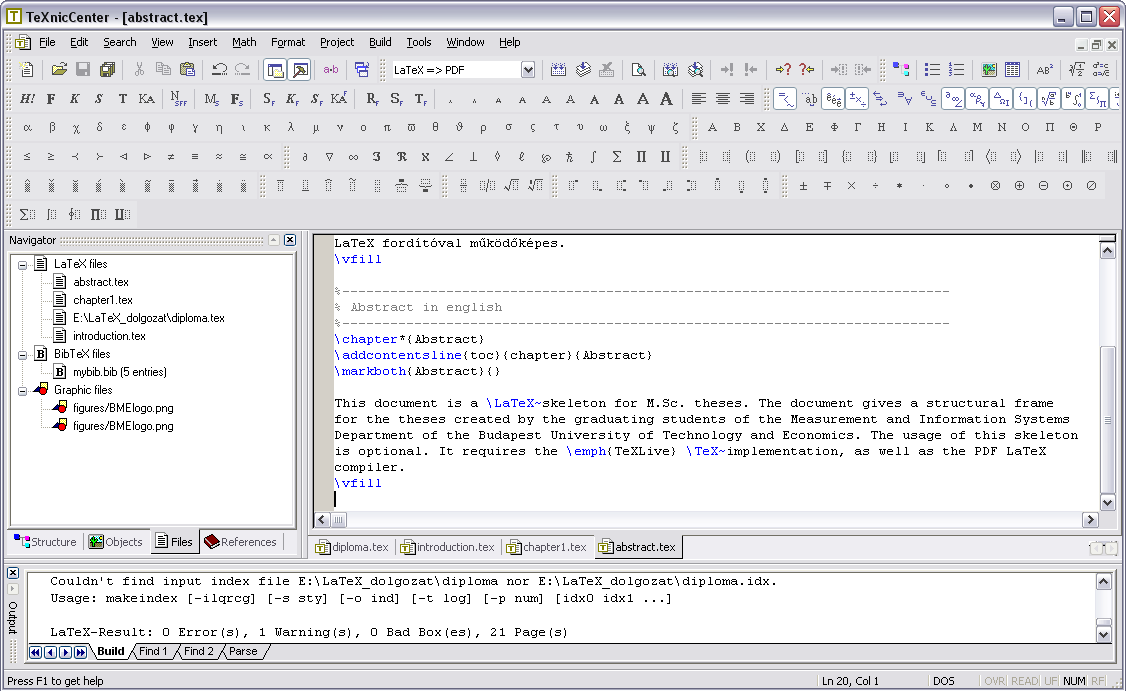
\includegraphics[width=150mm, keepaspectratio]{figures/TeXnicCenter.png}
\caption{A TeXnicCenter Windows alap� \LaTeX-szerkeszt�.} 
\label{fig:TexnicCenter}
\end{figure}

Egy m�sik haszn�lhat� Windows alap� szerkeszt�program a LEd (LaTeX Editor,\\\url{http://www.latexeditor.org/}), a TeXnicCenter azonban stabilabb, gyorsabb, �s jobban haszn�lhat�.

%----------------------------------------------------------------------------
\section{A dokumentum leford�t�sa Windows alatt}
%----------------------------------------------------------------------------
A TeXnicCenter �s a LEd kiz�r�lag szerkeszt�program (b�r az ut�bbiban DVI-n�zeget� is van), �gy a dokumentum ford�t�s�hoz sz�ks�ges eszk�z�ket nem tartalmazza. Windows alatt alapvet�en k�t lehet�s�g k�z�l �rdemes v�lasztani: MiKTeX (\url{http://miktex.org/}) �s TeXLive (\url{http://www.tug.org/texlive/}) programcsomag. Az ut�bbi m�k�dik Mac OS X, GNU/Linux alatt �s Unix-sz�rmaz�kokon is. A MiKTeX egy alapcsomag telep�t�se ut�n mindig let�lti a haszn�lt funkci�khoz sz�ks�ges, de lok�lisan hi�nyz� \TeX-csomagokat, m�g a TeXLive DVD ISO verz�ban f�rhet� hozz�. Ez a dokumentum TeXLive 2008 programcsomag seg�ts�g�vel fordult, amelynek DVD ISO verzi�ja a megadott oldalr�l let�lthet�. A sablon leford�t�s�hoz a disztrib�ci�ban szerepl� \verb+magyar.ldf+ f�jlt a \verb+http://www.math.bme.hu/latex/+ v�ltozatra kell cser�lni, vagy az ut�bbi v�ltozatot be kell m�solni a projekt-k�nyvt�rba (ahogy ezt meg is tett�k a sablonban) k�l�nben anom�li�k tapasztalhat�k a dokumentumban (pl. az �bra- �s t�bl�zat-al��r�sok form�tuma nem a be�ll�tott lesz, vagy bizonyos oldalakon megjelenik alap�telmez�sben egy fejl�c). A TeXLive 2008-at m�g nem kell k�l�n telep�teni a g�pre, elegend� DVD-r�l (vagy az ISO f�jlb�l k�zvetlen�l, pl. DaemonTools-szal) haszn�lni. 

A \TeX-eszk�z�ket tartalmaz� programcsomag bin�risainak el�r�si �tj�t minden esetben be kell �ll�tani a szerkeszt�programban, p�ld�ul TeXnicCenter eset�n legegyszer�bben a \verb+Build / Define output profiles...+ men�ponttal el�h�vott dial�gusablakban a \verb+Wizard...+ gombra kattintva tehetj�k ezt meg.

A PDF-\LaTeX~haszn�lata eset�n a gener�lt dokumentum k�zvetlen�l PDF-form�tumban �ll rendelkez�sre. Amennyiben a PDF-f�jl egy PDF-n�z�ben (pl. Adobe Acrobat Reader vagy Foxit PDF Reader) meg van nyitva, akkor a f�jlle�r�t a PDF-n�z� program tipikusan lefoglalja. Ilyen esetben a dokumentum �jraford�t�sa hiba�zenettel kil�p. Ha bez�rjuk �s �jra megnyitjuk a PDF dokumentumot, akkor pedig a PDF-n�z�k t�bbs�ge az els� oldalon nyitja meg a dokumentumot, nem a legut�bb olvasott oldalon. Ezzel szemben p�ld�ul az egyszer� �s ingyenes \textcolor{blue}{Sumatra PDF} nev� program k�pes arra, hogy a megnyitott dokumentum megv�ltoz�s�t detekt�lja, �s friss�tse a n�zetet az aktu�lis oldal megtart�s�val.

%----------------------------------------------------------------------------
\section{Eszk�z�k Linuxhoz}
%----------------------------------------------------------------------------
Linux oper�ci�s rendszer alatt is rengeteg szerkeszt�program van, pl. a KDE alap� Kile j�l haszn�lhat�. Ez ingyenesen let�lthet�, vagy �ppens�ggel az adott Linux-disztrib�ci� eleve tartalmazza, ahogyan a dokumentum ford�t�s�hoz sz�ks�ges csomagokat is. Az Ubuntu Linux disztrib�ci�k alatt p�ld�ul legt�bbsz�r a \verb+texlive-base+ csomag telep�t�s�vel haszn�lhat�k a \LaTeX-eszk�z�k.


\setcounter{chapter}{2}
%----------------------------------------------------------------------------
\chapter*{2. Tétel}
%----------------------------------------------------------------------------

\textbf{Témakörök:} A lineáris programozás alapfeladata, kétváltozós feladat grafikus megoldása. Lineáris egyenlőtlenség-rendszer megoldása Fourier-Motzkin eliminációval.

\noindent\hrulefill

\section*{LP feladatok alakjai}

\begin{theo} TODO \end{theo}

\section*{Dualitás tétel}

\begin{theo} 
Ha a $max \lbrace c x: Ax\leq b\rbrace$ primál program megoldható és felülről korlátos:
\begin{enumerate}
\item	a $min \lbrace yb: yA=c,y\geq 0\rbrace$ duális program is megoldható és alulról korlátos,
\item	a primál programnak létezik maximuma és a duális programnak létezik minimuma,
\item	továbbá ezek megegyeznek: $max\lbrace cx: Ax\leq b\rbrace = min\lbrace yb: yA=c,y\geq 0\rbrace$
\end{enumerate}
\end{theo}
Megjegyzés: $(2)$-re szükség van, mert egy számhalmaz felülről korlátosságából általában nem következik, hogy létezik maximuma.

\section*{Ekvivalens alak}
\begin{theo}
Ha a $max\lbrace cx:AX\leq b,x\geq 0\rbrace$ primál program megoldható és felülről korlátos:
\begin{enumerate}
\item a $min \lbrace yb:yA\geq c, y \geq 0\rbrace$ duális program is megoldható és alulról korlátos,
\item	a primál programnak létezik maximuma és a duális programnak létezik minimuma,
\item	továbbá ezek megegyeznek: $max\lbrace cx:AX\leq b,x\geq 0\rbrace = min \lbrace yb:yA\geq c, y \geq 0\rbrace$
\end{enumerate}
\end{theo}

\newpage

\section*{Bonyolultság}
\subsection*{LP feladat, eldöntési problémaként megfogalmazva}
Van-e az $Ax\leq b$ feltételt kielégítő $x$ vektorok között olyan, amelyre $cx\geq t$?
\begin{itemize}
	\item NP-beli: tanú egy ilyen $x$
	\item co-NP-beli: ha $cx<t$, akkor a duális megoldása ($y$) tanú erre
	\item (a tanúk polinomiális méretűek)
\end{itemize}

\subsection*{Módszerek}
\begin{itemize}
\item Szimplex módszer (1947, Dantzig): nem polinomiális, de a gyakorlati alkalmazások során gyors
\item Ellipszoid módszer (1979, Hacsijan): polinomiális, de a gyakorlati alkalmazások során lassú
\item Belső pontos módszerek (1984, Karmarkar): polinomiális, a gyakorlati alkalmazások során eredményes, de nem elterjedt
\end{itemize}


\setcounter{chapter}{3}
%----------------------------------------------------------------------------
\chapter*{3. Tétel}
%----------------------------------------------------------------------------

\textbf{Témakörök:} Farkas-lemma (két alakban). A lineáris program célfüggvénye felülről korlátosságának feltételei.

\noindent\hrulefill

\section*{Farkas-lemma 1.}
Tetszőleges $A$, $b$ esetén az alábbi rendszerek közül pontosan az egyiknek van megoldása:
\begin{itemize}
\item (1) $Ax\leq b$
\item (2) $yA=0$, $y\geq 0$, $yb<0$
\end{itemize}

\section*{Farkas-lemma 2.}
Tetszőleges $A$, $b$ esetén az alábbi rendszerek közül pontosan az egyiknek van megoldása:
\begin{itemize}
\item (1) $Ax=b$, $x\geq 0$
\item (2) $yA\geq 0$, $yb<0$
\end{itemize}

\textbf{Megjegyzés:} a tétel (1) állítása felfogható egyenlőtlenség rendszerként is: $Ax\leq b$, $(-A)x\leq (-b)$, $(-E)x\leq 0$. Erre is alkalmazható a Farkas-lemma 1. alakja.

\section*{Következmény}
Tetszőleges $A$, $b$ esetén az alábbi rendszerek közül pontosan az egyiknek van megoldása:
\begin{itemize}
\item (1) $Ax=b$
\item (2) $yA=0$, $yb\neq 0$
\end{itemize}

\section*{Célfüggvény korlátossága}
Tegyük fel, hogy $Ax\leq b$ megoldható, $c$ tetszőleges adott vektor. Ekkor az alábbi állítások ekvivalensek:
\begin{itemize}
\item (1) az $Ax\leq b$ megoldáshalmazán $cx$ felülről korlátos,
\item (2) nincs megoldása az $Az\leq 0$, $cz>0$ rendszernek,
\item (3) van megoldása az $yA=c$, $y\geq 0$ rendszernek.
\end{itemize}

\setcounter{chapter}{4}
%----------------------------------------------------------------------------
\chapter*{4. Tétel}
%----------------------------------------------------------------------------

\textbf{Témakörök:} A lineáris programozás dualitástétele (két alakban). A lineáris programozás alapfeladatának bonyolultsága (biz. nélkül).

\noindent\hrulefill

\section*{LP feladatok alakjai}
Drakula Művek példája $c=(12,12)$ célfüggvény mellett:

\begin{figure}[h!]
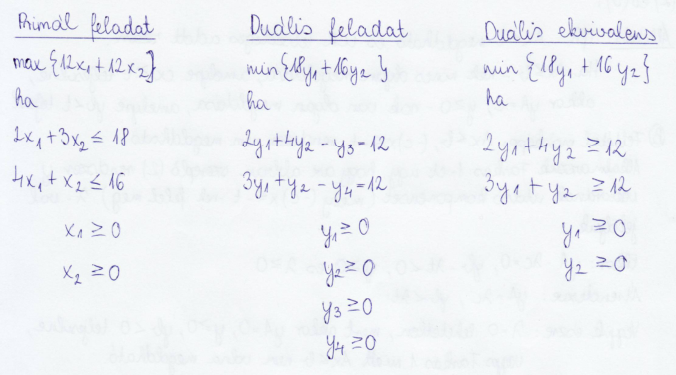
\includegraphics[width=14cm]{lp_alakok}
\centering
\end{figure}

\textbf{Megjegyzés:} $y_{3}$ és $y_{4}$ elhagyása a rendszerből nem befolyásolja a megoldhatóságot, sem a célfüggvényértéket. Az ekvivalens alak már könnyen ábrázolható grafikusan a síkon. Ha a primál feladatban elő van írva a változók nemnegatív értékűsége, akkor a duális esetében sem szabad erről megfeledkezni!

\section*{Dualitás tétel}

\begin{theo} 
Ha a $max \lbrace c x: Ax\leq b\rbrace$ primál program megoldható és felülről korlátos:
\begin{enumerate}
\item	a $min \lbrace yb: yA=c,y\geq 0\rbrace$ duális program is megoldható és alulról korlátos,
\item	a primál programnak létezik maximuma és a duális programnak létezik minimuma,
\item	továbbá ezek megegyeznek: $max\lbrace cx: Ax\leq b\rbrace = min\lbrace yb: yA=c,y\geq 0\rbrace$
\end{enumerate}
\end{theo}
\textbf{Megjegyzés:} $(2)$-re szükség van, mert egy számhalmaz felülről korlátosságából általában nem következik, hogy létezik maximuma.

\section*{Ekvivalens alak}
\begin{theo}
Ha a $max\lbrace cx:AX\leq b,x\geq 0\rbrace$ primál program megoldható és felülről korlátos:
\begin{enumerate}
\item a $min \lbrace yb:yA\geq c, y \geq 0\rbrace$ duális program is megoldható és alulról korlátos,
\item	a primál programnak létezik maximuma és a duális programnak létezik minimuma,
\item	továbbá ezek megegyeznek: $max\lbrace cx:AX\leq b,x\geq 0\rbrace = min \lbrace yb:yA\geq c, y \geq 0\rbrace$
\end{enumerate}
\end{theo}

\section*{Bonyolultság}
\subsection*{LP feladat, eldöntési problémaként megfogalmazva}
Van-e az $Ax\leq b$ feltételt kielégítő $x$ vektorok között olyan, amelyre $cx\geq t$?
\begin{itemize}
	\item NP-beli: tanú egy ilyen $x$
	\item co-NP-beli: ha $cx<t$, akkor a duális megoldása ($y$) tanú erre
	\item (a tanúk polinomiális méretűek)
\end{itemize}

\subsection*{Módszerek}
\begin{itemize}
\item Szimplex módszer (1947, Dantzig): nem polinomiális, de a gyakorlati alkalmazások során gyors
\item Ellipszoid módszer (1979, Hacsijan): polinomiális, de a gyakorlati alkalmazások során lassú
\item Belső pontos módszerek (1984, Karmarkar): polinomiális, a gyakorlati alkalmazások során eredményes, de nem elterjedt
\end{itemize}


\setcounter{chapter}{5}
%----------------------------------------------------------------------------
\chapter*{5. Tétel}
%----------------------------------------------------------------------------

\textbf{Témakörök:} Egészértékű programozás: a feladat bonyolultsága, korlátozás és szétválasztás (Branch and Bound). Totálisan unimoduláris mátrix fogalma, példák. Egészértékű programozás totálisan unimoduláris együtthatómátrixszal (biz. nélkül).

\noindent\hrulefill

\section*{LP feladatok alakjai}

\begin{theo} TODO \end{theo}

\section*{Dualitás tétel}

\begin{theo} 
Ha a $max \lbrace c x: Ax\leq b\rbrace$ primál program megoldható és felülről korlátos:
\begin{enumerate}
\item	a $min \lbrace yb: yA=c,y\geq 0\rbrace$ duális program is megoldható és alulról korlátos,
\item	a primál programnak létezik maximuma és a duális programnak létezik minimuma,
\item	továbbá ezek megegyeznek: $max\lbrace cx: Ax\leq b\rbrace = min\lbrace yb: yA=c,y\geq 0\rbrace$
\end{enumerate}
\end{theo}
Megjegyzés: $(2)$-re szükség van, mert egy számhalmaz felülről korlátosságából általában nem következik, hogy létezik maximuma.

\section*{Ekvivalens alak}
\begin{theo}
Ha a $max\lbrace cx:AX\leq b,x\geq 0\rbrace$ primál program megoldható és felülről korlátos:
\begin{enumerate}
\item a $min \lbrace yb:yA\geq c, y \geq 0\rbrace$ duális program is megoldható és alulról korlátos,
\item	a primál programnak létezik maximuma és a duális programnak létezik minimuma,
\item	továbbá ezek megegyeznek: $max\lbrace cx:AX\leq b,x\geq 0\rbrace = min \lbrace yb:yA\geq c, y \geq 0\rbrace$
\end{enumerate}
\end{theo}

\newpage

\section*{Bonyolultság}
\subsection*{LP feladat, eldöntési problémaként megfogalmazva}
Van-e az $Ax\leq b$ feltételt kielégítő $x$ vektorok között olyan, amelyre $cx\geq t$?
\begin{itemize}
	\item NP-beli: tanú egy ilyen $x$
	\item co-NP-beli: ha $cx<t$, akkor a duális megoldása ($y$) tanú erre
	\item (a tanúk polinomiális méretűek)
\end{itemize}

\subsection*{Módszerek}
\begin{itemize}
\item Szimplex módszer (1947, Dantzig): nem polinomiális, de a gyakorlati alkalmazások során gyors
\item Ellipszoid módszer (1979, Hacsijan): polinomiális, de a gyakorlati alkalmazások során lassú
\item Belső pontos módszerek (1984, Karmarkar): polinomiális, a gyakorlati alkalmazások során eredményes, de nem elterjedt
\end{itemize}


\setcounter{chapter}{6}
%----------------------------------------------------------------------------
\chapter*{6. Tétel}
%----------------------------------------------------------------------------

\textbf{Témakörök:} A lineáris és egészértékű programozás alkalmazása páros gráfokra és intervallumrendszerekre: Egerváry tétele, intervallumrendszerek egyenletes színezése.

\noindent\hrulefill

\begin{defn} [Illeszkedési mátrix] Legyen $n$ pontú gráfnak $e$ éle és definiáljuk az $n\times e$ méretű $B(G)=b_{ij}$ mátrix elemeit, hogy: \end{defn}

\begin{theo} Minden irányított gráf illeszkedési mátrixa TU. \end{theo}

\begin{prf} [Teljes indukció] 
Válasszunk $M$ $k\times k$-as részmátrixot.
\begin{itemize}
	\item ha $k=1$, akkor nyilvánvaló az állítás, hisz minden elem $0$ vagy $\pm 1$
	\item ha $k\geq 2$ és:
	\begin{itemize}
		\item $M$-nek van olyan oszlopa, melyben legfeljebb egy nemnulla elem van, akkor fejtsük ki $detM$-et eszerint az oszlop szerint, ekkor az indukciós feltétel szerint készen vagyunk.
		\item egyébként minden oszlopban egy $+1$ és egy $-1$ elem van, ekkor $M$ sorainak összege nullvektor, a determináns $0$.
	\end{itemize}
\end{itemize}
\end{prf}

\begin{theo} Páros gráf illeszkedési mátrixa TU. \end{theo}

\begin{prf}
Irányítsuk $G(A,B,E)$ páros gráf éleit úgy, hogy minden él A-ból B-be mutasson. Ekkor az előző tétel szerint $B(G)$ TU. A B-hez tartozó sorokat szorozzuk $-1$-gyel, de ez nem változtat TU tulajdonságon.
\end{prf}


\setcounter{chapter}{7}
%----------------------------------------------------------------------------
\chapter*{7. Tétel}
%----------------------------------------------------------------------------

\textbf{Témakörök:} A lineáris és egészértékű programozás alkalmazása hálózati folyamproblémákra: a maximális folyam, a minimális költségű folyam és a többtermékes folyam feladatai, ezek hatékony megoldhatósága a tört-, illetve egészértékű esetben.

\noindent\hrulefill

\section*{LP feladatok alakjai}

\begin{theo} TODO \end{theo}

\section*{Dualitás tétel}

\begin{theo} 
Ha a $max \lbrace c x: Ax\leq b\rbrace$ primál program megoldható és felülről korlátos:
\begin{enumerate}
\item	a $min \lbrace yb: yA=c,y\geq 0\rbrace$ duális program is megoldható és alulról korlátos,
\item	a primál programnak létezik maximuma és a duális programnak létezik minimuma,
\item	továbbá ezek megegyeznek: $max\lbrace cx: Ax\leq b\rbrace = min\lbrace yb: yA=c,y\geq 0\rbrace$
\end{enumerate}
\end{theo}
Megjegyzés: $(2)$-re szükség van, mert egy számhalmaz felülről korlátosságából általában nem következik, hogy létezik maximuma.

\section*{Ekvivalens alak}
\begin{theo}
Ha a $max\lbrace cx:AX\leq b,x\geq 0\rbrace$ primál program megoldható és felülről korlátos:
\begin{enumerate}
\item a $min \lbrace yb:yA\geq c, y \geq 0\rbrace$ duális program is megoldható és alulról korlátos,
\item	a primál programnak létezik maximuma és a duális programnak létezik minimuma,
\item	továbbá ezek megegyeznek: $max\lbrace cx:AX\leq b,x\geq 0\rbrace = min \lbrace yb:yA\geq c, y \geq 0\rbrace$
\end{enumerate}
\end{theo}

\newpage

\section*{Bonyolultság}
\subsection*{LP feladat, eldöntési problémaként megfogalmazva}
Van-e az $Ax\leq b$ feltételt kielégítő $x$ vektorok között olyan, amelyre $cx\geq t$?
\begin{itemize}
	\item NP-beli: tanú egy ilyen $x$
	\item co-NP-beli: ha $cx<t$, akkor a duális megoldása ($y$) tanú erre
	\item (a tanúk polinomiális méretűek)
\end{itemize}

\subsection*{Módszerek}
\begin{itemize}
\item Szimplex módszer (1947, Dantzig): nem polinomiális, de a gyakorlati alkalmazások során gyors
\item Ellipszoid módszer (1979, Hacsijan): polinomiális, de a gyakorlati alkalmazások során lassú
\item Belső pontos módszerek (1984, Karmarkar): polinomiális, a gyakorlati alkalmazások során eredményes, de nem elterjedt
\end{itemize}


\setcounter{chapter}{8}
%----------------------------------------------------------------------------
\chapter*{8. Tétel}
%----------------------------------------------------------------------------

\textbf{Témakörök:} Matroid definíciója, alapfogalmak (bázis, rang, kör). Példák: lineáris matroid (mátrixmatroid), grafikus matroid, uniform matroid. A rangfüggvény szubmodularitása.

\noindent\hrulefill

\section*{LP feladatok alakjai}

\begin{theo} TODO \end{theo}

\section*{Dualitás tétel}

\begin{theo} 
Ha a $max \lbrace c x: Ax\leq b\rbrace$ primál program megoldható és felülről korlátos:
\begin{enumerate}
\item	a $min \lbrace yb: yA=c,y\geq 0\rbrace$ duális program is megoldható és alulról korlátos,
\item	a primál programnak létezik maximuma és a duális programnak létezik minimuma,
\item	továbbá ezek megegyeznek: $max\lbrace cx: Ax\leq b\rbrace = min\lbrace yb: yA=c,y\geq 0\rbrace$
\end{enumerate}
\end{theo}
Megjegyzés: $(2)$-re szükség van, mert egy számhalmaz felülről korlátosságából általában nem következik, hogy létezik maximuma.

\section*{Ekvivalens alak}
\begin{theo}
Ha a $max\lbrace cx:AX\leq b,x\geq 0\rbrace$ primál program megoldható és felülről korlátos:
\begin{enumerate}
\item a $min \lbrace yb:yA\geq c, y \geq 0\rbrace$ duális program is megoldható és alulról korlátos,
\item	a primál programnak létezik maximuma és a duális programnak létezik minimuma,
\item	továbbá ezek megegyeznek: $max\lbrace cx:AX\leq b,x\geq 0\rbrace = min \lbrace yb:yA\geq c, y \geq 0\rbrace$
\end{enumerate}
\end{theo}

\newpage

\section*{Bonyolultság}
\subsection*{LP feladat, eldöntési problémaként megfogalmazva}
Van-e az $Ax\leq b$ feltételt kielégítő $x$ vektorok között olyan, amelyre $cx\geq t$?
\begin{itemize}
	\item NP-beli: tanú egy ilyen $x$
	\item co-NP-beli: ha $cx<t$, akkor a duális megoldása ($y$) tanú erre
	\item (a tanúk polinomiális méretűek)
\end{itemize}

\subsection*{Módszerek}
\begin{itemize}
\item Szimplex módszer (1947, Dantzig): nem polinomiális, de a gyakorlati alkalmazások során gyors
\item Ellipszoid módszer (1979, Hacsijan): polinomiális, de a gyakorlati alkalmazások során lassú
\item Belső pontos módszerek (1984, Karmarkar): polinomiális, a gyakorlati alkalmazások során eredményes, de nem elterjedt
\end{itemize}


\setcounter{chapter}{9}
%----------------------------------------------------------------------------
\chapter*{9. Tétel}
%----------------------------------------------------------------------------

\textbf{Témakörök:} Mohó algoritmus matroidon. Matroid megadása rangfüggvényével, bázisaival (biz. nélkül). Matroid duálisa, a duális matroid rangfüggvénye.

\noindent\hrulefill

\section*{Mohó algoritmus (röviden)}

Legyen $M=(E,F)$ matroid, $w:E\rightarrow \mathbb{R}_{+}$ nemnegatív súlyfüggvény. Keressük a maximális összsúlyú független halmazt, azaz: $\max\limits_{X\in F} \sum\limits_{e\in X} w(e)$.\\
A mohó algoritmus tetszőleges matroidra és súlyfüggvényre optimális (maximális összsúlyú) megoldást ad.

\section*{Matroid megadása}

Függetlenségi axiómákkal (lásd: előző tétel).

\section*{Megadás bázisokkal}
\begin{itemize}
\item (B1) $B\neq\emptyset$,
\item (B2) $|X_{1}| = |X_{2}|$ minden $X_{1},X_{2}\in B$-re,
\item (B3) ha $X_{1},X_{2}\in B$ és $e_{1}\in X_{1}$, akkor létezik olyan $e_{2}\in X_{2}$, melyre $X_{1}-e_{1}+e_{2}\in B$.
\end{itemize}
Fordítva: ha $(E,B)$ egy halmazrendszer a (B1), (B2) és (B3) tulajdonságokkal, akkor $M=(E,F)$ matroidot alkot, ahol: $F=\lbrace H:H\subseteq B\rbrace$ valamely $B\in B$-re.

\section*{Megadás rangfüggvénnyel}
Lásd: korábban

\section*{Egyéb fogalmak}
\begin{defn} [Lezárt]
$(E,F)$ matroidban egy $X\subseteq E$ halmaz lezártja egy maximális olyan halmaz, mely tartalmazza $X$-et és rangja megegyezik $X$ rangjával. Jele: $\overline{X}$.
\end{defn}

\begin{defn} [Zárt halmaz]
egy $X$ halmaz zárt, ha $X=\overline{X}$.
\end{defn}

\begin{defn} [Izomorfia]
Két matroid izomorf, ha létezik olyan bijekció a két alaphalmaz között, mely független halmazt független halmazba visz. Jele: $M\equiv M^{'}$.
\end{defn}

\section*{Duális}
$M=(E,F)$, és $M$ duálisának alaphalmaza legyen $E$, és egy $X\subseteq E$ halmaz akkor legyen az új halmazrendszer eleme, ha $E-X$ tartalmaz $M$-beli bázist. Ezt a halmazt jelöljük $F^{*}$-al.

\begin{defn}
$M=(E,F)$ matroid bázisai $B=\lbrace B_{1},B_{2},\cdots ,E-B_{n}\rbrace$. Ebből már adódik $F^{*}$.
\end{defn}

\begin{theo} [Duális matroid tétel] Az $M^{*} =(E,F^{*})$ matroid.\\
FYI: $(M^{*})^{*}\equiv M$
\end{theo}

\subsection*{Példa}
$M=U_{5,2}$:
\begin{itemize}
\item $M$-ben minden legfeljebb 2-elemű halmaz független,
\item a duálisban azon halmazok függetlenek, amelyek komplementerei tartalmaznak $M$-beli bázist, azaz 2-elemű halmazt,
\item ezek a legfeljebb 3-elemű halmazok, tehát $M^{*}=U_{5,3}$.
\end{itemize}

\subsection*{Duális rangfüggvény}
$r^{*}(X)=|X|-r(E)+r(E-X)$

\setcounter{chapter}{10}
%----------------------------------------------------------------------------
\chapter*{10. Tétel}
%----------------------------------------------------------------------------

\textbf{Témakörök:} Elhagyás és összehúzás. Matroidok direkt összege, összefüggősége. $T$ test felett reprezentálható matroid duálisának $T$ feletti reprezentálhatósága.

\noindent\hrulefill

\section*{Elhagyás/törlés}



\section*{Összehúzás}



\section*{Direkt összeg}



\section*{Összefüggőség}



\section*{T-test feletti reprezentáció}

\subsection*{Konstrukció}


\setcounter{chapter}{11}
%----------------------------------------------------------------------------
\chapter*{11. Tétel}
%----------------------------------------------------------------------------

\textbf{Témakörök:} Grafikus, kografikus, reguláris, bináris és lineáris matroid fogalma, ezek kapcsolata (ebből bizonyítás csak a grafikus és reguláris matroidok közötti kapcsolatra), példák. Fano-matroid, példa nemlineáris matroidra. Bináris, reguláris és grafikus matroidok jellemzése tiltott minorokkal: Tutte tételei (biz. nélkül).

\noindent\hrulefill

\section*{Matroid osztályok}
\textbf{Grafikus vagy körmatroid:} $G$ gráf által indukált matroid, melyben $E=\lbrace G$ élei$\rbrace$, $F=\lbrace G$-beli erdők$\rbrace$.\\
\textbf{Kografikus:} grafikus matroid duálisa kografikus.\\
\textbf{Reguláris:} tetszőleges test felett reprezentálható.\\
\textbf{Bináris:} a kételemű (bináris) test felett reprezentálható.\\
\textbf{Lineáris:} van olyan test, ami felett reprezentálható.\\ 

\begin{figure}[h!]
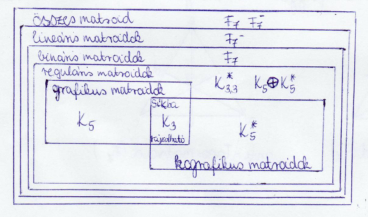
\includegraphics{matroid_osztalyok}
\centering
\end{figure}

\begin{theo}
Grafikus matroid bármely test felett reprezentálható (reguláris).
\end{theo}

\begin{theo}
Ha $M=(E,F)$ reprezentálható az $F$ test felett, akkor $M^{*}$ is. $\Rightarrow$ A kografikus matroidok is regulárisak!
\end{theo}

\section*{Karakterisztika}
Ha az $F$ testhez van olyan pozitív egész $k$, melyre teljesül, hogy az $x+x+\cdots +x$ ($k$ tagú) összeg értéke minden $x\in F$ elemre zérus, akkor a legkisebb ilyen $k$ szám a test karakterisztikája. (Minden véges testnek van karakterisztikája, ami mindig egy prím.)

\section*{Fano matroid}
Adott a hételemű halmaz: $\lbrace a,b,c,d,e,f,g \rbrace$.
\begin{itemize}
\item minden legfeljebb kételemű halmaz független
\item minden legalább négyelemű halmaz összefüggő
\item a háromeleműek közül azok függetlenek, melyeket nem köt össze vonal az ábrán
\end{itemize}

\begin{figure}[h!]
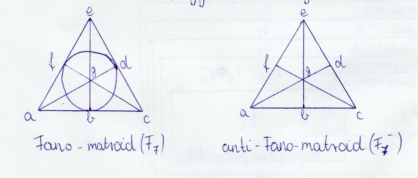
\includegraphics{fano_matroid}
\centering
\end{figure}

\section*{Tutte tételei}
\begin{itemize}
\item $M$ matroid bináris $\Leftrightarrow$ nem tartalmaz minorként $U_{4,2}$ matroidot.
\item $M$ matroid reguláris $\Leftrightarrow$ nem tartalmaz minorként $U_{4,2}$, $F_{7}$ és $F_{7}^{*}$ matroidokat.
\item $M$ matroid grafikus $\Leftrightarrow$ nem tartalmaz minorként $U_{4,2}$; $F_{7}$, $F_{7}^{*}$, $M^{*}(K_{5})$ és $M^{*}(K_{3,3})$ matroidokat.
\end{itemize}

\setcounter{chapter}{12}
%----------------------------------------------------------------------------
\chapter*{12. Tétel}
%----------------------------------------------------------------------------

\textbf{Témakörök:} Matroidok összege. $k$-matroid metszet probléma, ennek bonyolultsága $k\geq3$ esetén.

\noindent\hrulefill

\section*{Matroidok összege}
$M_{1}=(E,F_{1})$ és $M_{2}=(E,F_{2})$ matroidok összege $M_{1}\vee M_{2}=(E,F^{'})$, ahol $X\in F^{'}\Leftrightarrow\exists X_{1},X_{2}$, hogy $X=X_{1}\cup X_{2}$ és $X_{1}\in F_{1}$, valamint $X_{2}\in F_{2}$. (Azaz előáll egy $F_{1}$-beli és egy $F_{2}$-beli elem uniójaként.)

\begin{theo} A függetlenségi aximómák segítségével bizonyítható, hogy matroidok összege is matroid. ($F(3)$-mat kell belátni.) \end{theo}

\section*{Matroidok metszete}
$M_{1}=(E,F_{1})$ és $M_{2}=(E,F_{2})$ matroidok metszete: $M_{1}\cap M_{2}=(E,F_{1}\cap F_{2})$ halmazrendszer.

\begin{theo} Két matroid metszete nem feltétlen matroid. \end{theo}

\section*{(Súlyozott) matroid metszet probléma (k-MMP vagy MMP\textsubscript{k})}
Két matroid metszetének egy minimális méretű vagy súlyú elemét keressük.\\
Adott: $k$ db matroid közös alaphalmazon: $M_{i}=(E,F_{i}), i=1,2,\ldots ,k$\\
Kérdés: létezik-e valamely konstans $p$-re $p$ méretű halmaz $\cap F_{i}$-ben?\\
Azaz: $\exists$-e $X\subseteq E: |X|\geq p: X\in \bigcap\limits_{i=1}^{k}F_{i}$

\section*{Bonyolultság}
\begin{itemize}
	\item $k=1,2$ esetén: polinomiális (Mohó algoritmus)
	\item $k\geq 3$ esetén: NP-teljes (Hamilton-út keresése)
\end{itemize}


\setcounter{chapter}{13}
%----------------------------------------------------------------------------
\chapter*{13. Tétel}
%----------------------------------------------------------------------------

\textbf{Témakörök:} A $k$-matroid partíciós probléma, ennek algoritmikus megoldása. A 2-matroid-metszet feladat visszavezetése matroid partíciós problémára.

\noindent\hrulefill

\section*{LP feladatok alakjai}

\begin{theo} TODO \end{theo}

\section*{Dualitás tétel}

\begin{theo} 
Ha a $max \lbrace c x: Ax\leq b\rbrace$ primál program megoldható és felülről korlátos:
\begin{enumerate}
\item	a $min \lbrace yb: yA=c,y\geq 0\rbrace$ duális program is megoldható és alulról korlátos,
\item	a primál programnak létezik maximuma és a duális programnak létezik minimuma,
\item	továbbá ezek megegyeznek: $max\lbrace cx: Ax\leq b\rbrace = min\lbrace yb: yA=c,y\geq 0\rbrace$
\end{enumerate}
\end{theo}
Megjegyzés: $(2)$-re szükség van, mert egy számhalmaz felülről korlátosságából általában nem következik, hogy létezik maximuma.

\section*{Ekvivalens alak}
\begin{theo}
Ha a $max\lbrace cx:AX\leq b,x\geq 0\rbrace$ primál program megoldható és felülről korlátos:
\begin{enumerate}
\item a $min \lbrace yb:yA\geq c, y \geq 0\rbrace$ duális program is megoldható és alulról korlátos,
\item	a primál programnak létezik maximuma és a duális programnak létezik minimuma,
\item	továbbá ezek megegyeznek: $max\lbrace cx:AX\leq b,x\geq 0\rbrace = min \lbrace yb:yA\geq c, y \geq 0\rbrace$
\end{enumerate}
\end{theo}

\newpage

\section*{Bonyolultság}
\subsection*{LP feladat, eldöntési problémaként megfogalmazva}
Van-e az $Ax\leq b$ feltételt kielégítő $x$ vektorok között olyan, amelyre $cx\geq t$?
\begin{itemize}
	\item NP-beli: tanú egy ilyen $x$
	\item co-NP-beli: ha $cx<t$, akkor a duális megoldása ($y$) tanú erre
	\item (a tanúk polinomiális méretűek)
\end{itemize}

\subsection*{Módszerek}
\begin{itemize}
\item Szimplex módszer (1947, Dantzig): nem polinomiális, de a gyakorlati alkalmazások során gyors
\item Ellipszoid módszer (1979, Hacsijan): polinomiális, de a gyakorlati alkalmazások során lassú
\item Belső pontos módszerek (1984, Karmarkar): polinomiális, a gyakorlati alkalmazások során eredményes, de nem elterjedt
\end{itemize}


\setcounter{chapter}{14}
%----------------------------------------------------------------------------
\chapter*{14. Tétel}
%----------------------------------------------------------------------------

\textbf{Témakörök:} $k$-polimatroid rangfüggvény fogalma. A 2-polimatroid-matching probléma, ennek bonyolultsága, Lovász tétele (biz. nélkül).

\noindent\hrulefill

\section*{k-polimatroid rangfüggvény}
$f:2^{E}\rightarrow \mathbb{N}$ egy k-polimatroid rangfüggvény, ha teljesülnek rá az alábbi axiómák:
\begin{itemize}
\item (1) $r(\emptyset )=0$,
\item (2) $r(\lbrace x\rbrace)\leq k$, $\forall x\in E$ elemre ,
\item (3) $X\subseteq Y \Rightarrow r(X)\leq r(Y)$,
\item (4) $r(X)+r(Y)\geq r(X\cap Y)+r(X\cup Y)$.
\end{itemize}
Általánosítása a matroid rangfüggvénynek, értsd:\\
$k=1$: speciális eset: $r(\lbrace x\rbrace )\leq 1$, ekkor $R$ egy matroid rangfüggvénye.\\
\textbf{Megjegyzés:} $r(\lbrace x\rbrace )\leq k$-val ekvivalens az $r(X)\leq k|X|$, illetve az $r(X\cap Y)\leq r(X)+k|Y|$ axióma.

\section*{k-polimatroid matching probléma (k-PMM)}
\begin{defn} $X\subseteq E$ k-polimatroid matching, ha $r(X)=k|X|$ egyenlőség fennáll.\end{defn}
\begin{defn} k-polimatroid matching probléma:\\
Adott: $r$ és $t\in \mathbb{N}$\\
Kérdés: van-e legalább $T$ elemű k-polimatroid matching?
\end{defn}

\subsection*{Speciális esetek}
\begin{itemize}
\item[•] Input: tetszőleges $G$ gráf, $t\in \mathbb{N}$. Kérdés: $\nu(G)\geq t$?\\
2-PMM-ként megfogalmazva: $r(X)=|X$ által lefedett pontok halmaza $|\leq 2|X|$\\
A 2-matching épp a közönséges párosításnak felel meg (innen az elnevezés).
\item[•] Input: két maroid, $t\in \mathbb{N}$. Kérdés: létezik-e $X\subseteq E$, $|X|\geq t$, $X\in F_{1}\cap F_{2}$ (matroid metszet probléma)?\\
2-PMM-ként megfogalmazva: $f(X)=r_{1}(X)+r_{2}(X)\leq 2|X|$
\item[•] Az utolsó két probléma közös speciális esete: páros gráfban $\nu (G)\geq t$?\\
Megoldás: a 2. probléma leképezése a 3.-ra:\\
$M_{1}$ grafikus matroidban $e_{1}$ és $e_{2}$ párhuzamos élek, ha $e_{1}$-nek és $e_{2}$-nek felül van egy közös pontja. $M_{2}$-t hasonlóan értelmezzük a páros gráf alsó ponthalmazán.
\end{itemize}

\subsection*{Bonyolultság}
\begin{itemize}
\item $k\geq 3$ eset: NP-nehéz, mert speciális esetként tartalmazza a k-MMP-t.
\item $k=2$ eset: "matroidpárosítási probléma", speciális esetként tartalmazza 2-MMP-t.
\end{itemize}

\begin{theo}
A matroidpárosítási probléma (2-PMM) teljes általánosságban nem oldható meg polinomidőben. A teljes általánosságban kifejezés a függvény megadási módjára vonatkozik: azt jelenti, hogy bármely $X\subseteq E$ részhalmazra egységnyi idő alatt megtudhatjuk $r(X)$ értékét, de ettől eltekintve a 2-polimatroid rangfüggvényről semmit sem tudunk.
\end{theo}


\section*{Lovász László tétele}
"Legfontosabb speciális eset."
\begin{theo}
Vegyünk egy $k\times 2n$ méretű valós $M$ mátrixot, oszlopai legyenek rendre $M=(a_{1},b_{1},a_{2},b_{2},\cdots ,a_{n},b_{b})$ majd definiáljunk az $I=\lbrace 1,2,\cdots ,n\rbrace$ indexhalmazon egy $r$ függvényt úgy, hogy $X\subseteq I$ esetén legyen $r(X)$ az $\cup_{i\in X}\lbrace a_{i},b_{i}\rbrace$ vektorhalmaz által kifeszített altér dimenziója. Könnyű látni, hogy ilyenkor $r$ egy 2-polimatroid rangfüggvény.
\end{theo}

\begin{theo}
A matroidpárosítási probléma polinomidőben megoldható, ha a 2-polimatroid rangfüggvény egy adott valós elemű $M$ mátrixból a fent leírt módon nyerhető.
\end{theo}
%\bibliography{mybib}
%\addcontentsline{toc}{chapter}{Irodalomjegyzék}
%\bibliographystyle{plain}

\label{page:last}
\end{document}